\begin{question}
Recall the men-women problem from exercise~\ref{ex:menWomenServer}.  Implement
a class to solve this problem, using semaphores internally.
\end{question}

%%%%%

\begin{answerI}
My code arranges for each round to proceed as follows, and as illustrated in
the sequence diagram below.
%
\begin{enumerate}
\item[1.] A man waits (on |roundOver|) for the previous round to complete,
  writes his name, signals to a woman (on |manWritten|), and waits (on
  |womanWritten|) for a signal back;

\item[2.] A woman waits (on |manWritten|) for a man, reads his name, writes her
name, and signals back (on |womanWritten|);

\item[3.] The man reads her name, and signals (on |roundOver|) to a man
  waiting for the next round.
\end{enumerate}
%
\begin{center}
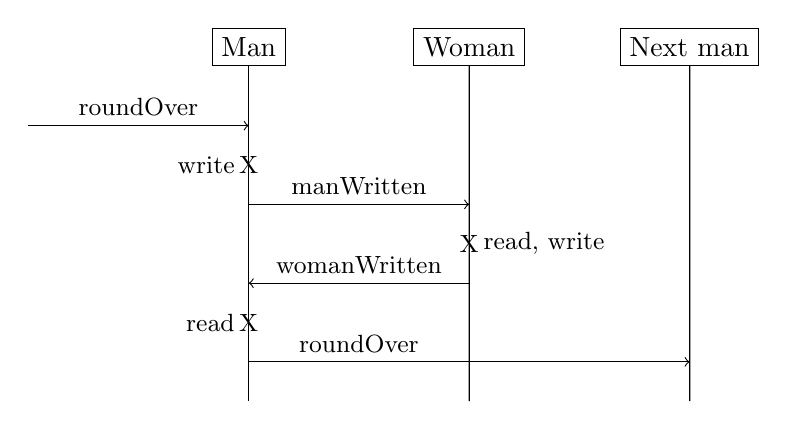
\begin{tikzpicture}[xscale = 1.4,yscale = 1.0]
\draw (0,0) node[draw](sender){Man};
\draw (2,0) node[draw](receiver){Woman};
\draw (4,0) node[draw](sender2){Next man};
\draw (sender) -- ++ (0,-4.5);
\draw (receiver) -- ++ (0,-4.5);
\draw (sender2) -- ++ (0,-4.5);
\draw[->] (-2.0,-1) -- 
  node[above] {\small\scalastyle roundOver} (0,-1);
\draw (0,-1.5) node{\small X}  node[left]{\small write\,};
\draw[->] (0,-2) -- node[above] { \small\scalastyle manWritten} (2,-2);
\draw (2,-2.5) node{\small X} node[right]{\,\small read, write};
\draw[<-] (0,-3) -- node[above] { \small\scalastyle womanWritten} (2,-3);
\draw (0,-3.5) node{\small X} node[left]{\small read\,};
\draw[->] (0,-4) -- node[above, near start] {\small\scalastyle roundOver} (4,-4);
\end{tikzpicture}
\end{center}
%
Of course, there are other orders one could choose.

The code is below, explained by comments.  The three semaphores collectively
ensure mutual exclusion. 
%
\begin{scala}
class MenWomenSemaphore extends MenWomenT{
  /** Name of the current (or last) woman. */
  private var woman = ""

  /** Name of the current (or last) man. */
  private var man = ""

  /** Semaphore where a man waits initially.  A signal indicates that the
    * previous round is over. */
  private val roundOver = new MutexSemaphore

  /** Semaphore where a woman waits until signalled.  A signal indicates that
    * the man has written his name. */
  private val manWritten = new SignallingSemaphore

  /** Semaphore where the current man waits for a woman.  A signal indicates
    * that a woman has written her name. */
  private val womanWritten = new SignallingSemaphore

  // The above three semaphores collectively ensure mutual exclusion.

  def manSync(me: String): String = {
    roundOver.down()    // Wait my turn (1).
    man = me            // Store my name.
    manWritten.up()     // Signal to a woman at (2).
    womanWritten.down() // Wait for an acknowledgement (3).
    val her = woman     // Get her name.
    roundOver.up()      // Signal to the next man at (1).
    her
  }

  def womanSync(me: String): String = {
    manWritten.down()         // Wait for a man (2).
    woman = me; val him = man // Store my name, get his.
    womanWritten.up()         // Signal to him at (3).
    him
  }
}
\end{scala}
\end{answerI}
